\documentclass[tikz]{standalone}
\usepackage{pgfplots}
\pgfplotsset{compat=1.15}
\usepackage{mathrsfs}
\usetikzlibrary{arrows,calc}
\usepackage{tkz-euclide}

\usepackage{fp}
\pagestyle{empty}

\definecolor{AngleClr}{rgb}{0,0.39215686274509803,0}
\definecolor{ShapeClr}{rgb}{0.6,0.2,0}

\begin{document}

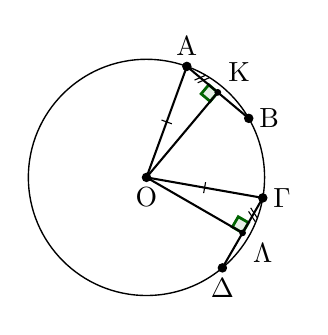
\begin{tikzpicture}[scale=.75]
\tkzSetUpLine[line width=1pt,color=black]
\tkzSetUpPoint[fill=black]

\tkzDefPoints{0/0/O,2/0/X}

\tkzDefPoint(30:2){B}
\tkzDefPoint(70:2){A}
\tkzDefPoint(-10:2){C}
\tkzDefPoint(-50:2){D}

\tkzDefPointBy[projection=onto A--B](O)\tkzGetPoint{K}
\tkzDefPointBy[projection=onto C--D](O)\tkzGetPoint{L}

\tkzMarkRightAngles[line width=1pt, size=.2,color=AngleClr,fill=AngleClr,fill opacity=0.1](O,K,A O,L,C)

\tkzDrawSegments[line width=0.75pt,color=black](O,A O,C A,B C,D O,K O,L)

\tkzDrawCircle[color=black,line width=0.5pt](O,X)

\tkzDrawPoints[size=3](A,B,O,C,D)
\tkzDrawPoints[size=2](K,L)
\tkzLabelPoint[above](A){$\rm A$}
\tkzLabelPoint[right](B){$\rm B$}
\tkzLabelPoint[right](C){$\rm \Gamma$}
\tkzLabelPoint[below](D){$\rm \Delta$}
\tkzLabelPoint[above right](K){$\rm K$}
\tkzLabelPoint[below right](L){$\rm \Lambda$}
\tkzLabelPoint[below](O){$\rm O$}

\tkzMarkSegments[mark=|,size=2](O,A O,C)
\tkzMarkSegments[mark=s||,size=2](K,A L,C)

\end{tikzpicture}

\end{document}
